\chapter{Grundlagen}
\section{Symmetrische Verschlüsselung}

Symmetrische Verschlüsselung basiert darauf, dass derselbe Schlüssel zum Ver- und Entschlüsseln verwendet wird.
Dementsprechend muss dieser Schlüssel dem Client und dem Server bekannt sein (siehe Abb. ~\ref{fig:symetric-crypto}).
  \begin{figure}[!htb]
    \center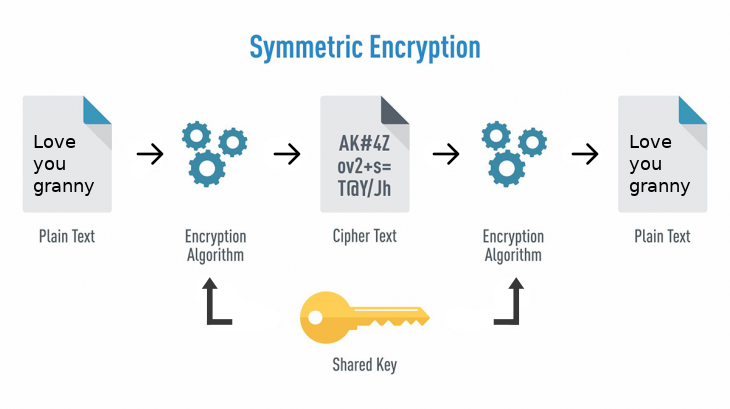
\includegraphics[scale=0.28]{images/symetric-crypto.png}
    \label{fig:symetric-crypto}
    \caption{Symmetrische Verschlüsselung}
  \end{figure}
    
\section{Asymmetrische Verschlüsselung}

Asymmetrische Verschlüsselung hingegen arbeitet auf einem öffentlichen und einem privaten Schlüssel. 
Hierbei wird der öffentliche zum Verschlüssen und der private zum Entschlüsseln verwendet.
Dadurch muss nur der private Schlüssel herausgegeben werden. (siehe Abb. ~\ref{fig:asymetric-crypto})
  \begin{figure}[!htb]
    \center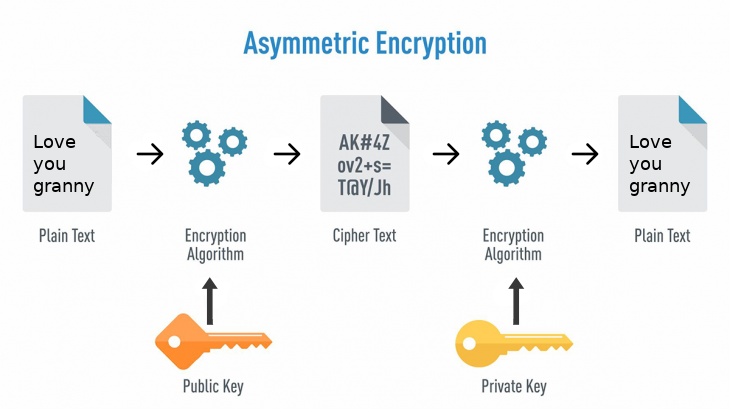
\includegraphics[scale=0.28]{images/asymetric-crypto.png}
    \caption{Asymmetrische Verschlüsselung}
    \label{fig:asymetric-crypto}
  \end{figure}

    
\section{Hash Funktionen}

Um eine große Eingabemenge auf eine kleine Zielmenge mit festgelgter Länge abzubilden, 
verwendet man sogenannte Hash Funktionen. Es gibt zahlreiche weitläufig bekannte Standards:
\begin{itemize}
    \item MD5
    \item Sha-2
    \item Argon
\end{itemize}
Eine besondere Kategorie nehmen die kryptographischen Funktionen ein: Hierbei geht es darum, eine 
Kollision zu vermeiden. Von einer Kollision wird gesprochen, wenn zwei unterschiedliche Eingabewerte zum selben Hash führen.

    
\section{Digitale Signaturen}

% TODO: Fix figure
Digitale Signature werden verwendet, um die Integrität und Authtenzität von Daten sicherzustellen. Eine Signatur ist für ein gegebenes Tupel aus
Daten und Schlüssel einzigartig. Wurde eine Nachricht entsprechend signiert, kann der Empfänger diese validieren. (siehe Abb. ~\ref{fig:signature})
\begin{figure}[!htb]
  \center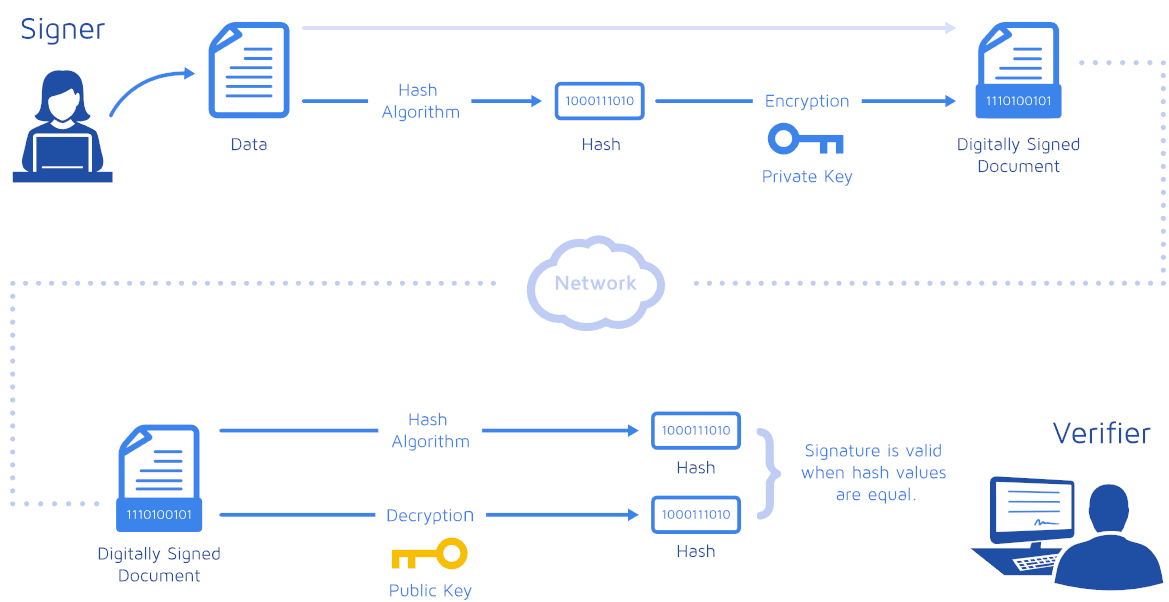
\includegraphics[scale=1.1]{images/signature-white.png}
  \label{fig:signature}
  \caption{Digitale Signatur}
\end{figure}

